\subsection{Moon Survival Prototype}

% objective of game (build base, need oxygen, survive, sandbox)
Moon Survival is a sandbox game based on the moon. The player controls a character stranded on the moon whose objective is to survive. The moon has no atmosphere, but the player's character requires air to survive. Therefore, he must construct a base and add oxygen generators inside of it. The basic physics of the game will cause the breathable air that is generated to diffuse throughout the base allowing the player to survive. The style of game is a creative open world in which to experiment, similar to Minecraft.\sidenote{Minecraft is a game about breaking and placing blocks. At first, people built structures to protect against nocturnal monsters, but as the game grew players worked together to create wonderful, imaginative things. See \url{https://minecraft.net/}} The player can build whatever and wherever they want to, and can experiment with oxygen diffusion physics.

There are two items available for the player to build: 

\begin{description}
\item[air generator] creates breathable air and releases it into its immediate surroundings. 
\item[wall] solid block that halts the diffusion of air as well as preventing the player from walking through that tile.
\end{description}
\noindent
Using only these two components the player must build their base in which their character is able to survive.

\begin{marginfigure}
	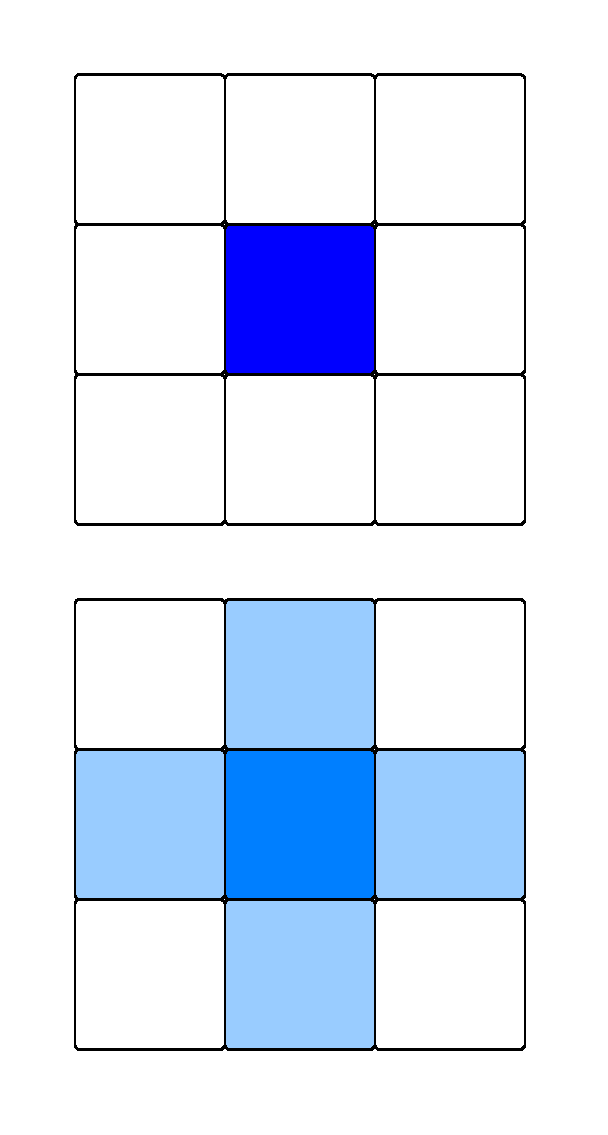
\includegraphics{res/space_base_prototype/MoonSurvivalAirDiffusion.pdf}
	\caption[Diffusion of air in Moon Survivial]{Diffusion of air through a 3x3 block layout. The greater the intensity of blue, the greater the concentration of air in that block. Air diffuses from the area of very high concentration in the centre block to its direct neighbours (the blocks to the North, South, East, and West).}
	\label{fig:SpaceBaseAirDiffusion}
\end{marginfigure}

% air physics (diffusion, dissapears at low quantities)
The physics of diffusion is highly simplified. The game is able to mimic the movement of air through the world without having to perform too many complex calculations. Figure~\ref{fig:SpaceBaseAirDiffusion} shows how air diffuses throughout a three by three area in one iteration of the game loop. The top diagram in the figure shows the state of the game prior to starting, and the bottom one shows how diffusion has occurred after one step. As shown, the air diffuses from an area of high concentration to areas of lower concentration.

The diffusion equation uses the following terms:
\begin{description}
\item[c] function from block to air concentration at that block
\item[t] diffusion rate, constant between 0 and 1 representing transfer rate, 0 is no transfer, 1 is transfer until equilibrium between blocks
\end{description}

For two adjacent blocks, $b_1$ and $b_2$, the volume of air that diffuses from $b_1$ to $b_2$ is:

$$ transfer = \frac{c(b_1) - c(b_2)}{2} * t $$
\noindent
Unfortunately, although this equation for diffusion allows for incredibly quick calculation, it has a problem due to its simplicity. The amount of air transferred from the centre block in Figure~\ref{fig:SpaceBaseAirDiffusion} reduces for each consecutive neighbour, i.e.\ the first neighbour gets more air than the second neighbour, and the second neighbour gets more air than the third neighbour, and so on, instead of all of the neighbours receiving the same degree of air transfer.

% controls (how to move about, collisions)

\begin{marginfigure}
	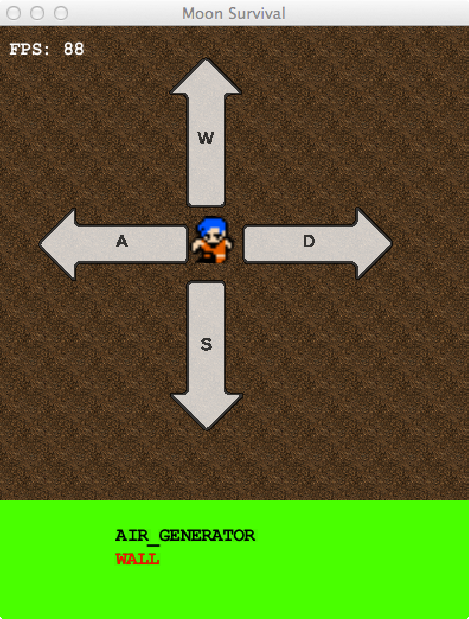
\includegraphics{res/space_base_prototype/MoonSurvivalControls.pdf}
	\caption{Overview of game controls in Moon Survival}
	\label{fig:SpaceBaseControls}
\end{marginfigure}

The game controls are extremely simple and will be familiar to most computer gamers. To move the character the player uses `w', `a', `s', and `d' to move North, West, South, and East respectively. Figure~\ref{fig:SpaceBaseControls} shows a screenshot of these movement controls within the game. If there is an obstacle in the way, such as a wall block, the player will be unable to move in that direction. A slight limitation of this movement system is that holding down a key does cause the player to continue to move in that direction. Instead the key must be repeatedly tapped to have this effect.

The player is equipped with one item (either `wall' or `air generator') at a time, and can switch between the items with the tab key. The currently selected item is displayed in the command bar at the base of the screen. To place an item, the player uses the space bar. This will place the item directly in front of player. If this block directly in front of the player is already filled with the currently selected item then it will be removed. For example, if the player is standing in front of a wall and the wall item is selected, then that wall will be removed if the player were to press the space bar.

\begin{marginfigure}
	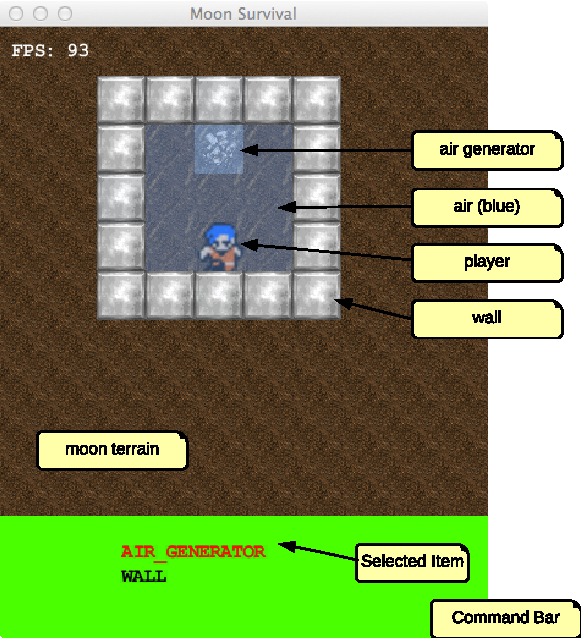
\includegraphics{res/space_base_prototype/MoonSurvivalGUI.pdf}
	\caption{Layout of the Moon Survival GUI}
	\label{fig:SpaceBaseGUI}
\end{marginfigure}

% GUI description (what each thing on screen is)
The GUI is described in the annotated screenshot shown in Figure~\ref{fig:SpaceBaseGUI}. The window is broken down into two panes: the game panel and the command panel. The game panel displays the player and their immediate surroundings. The command panel displays the items that the player has access to. The currently selected item is highlighted in red.

% conclusion (what aspects liked, what aspects were missing, etc)
Although this is a relatively simplistic game it helped get in the mindset of game design and development. It showed that the open world sandbox style game is entertaining even when it is so basic. However, playing the game also highlighted a missing aspect, danger. There are no other dangers in the game, such as monsters, to threaten the survival of the player. If there was a greater sense of danger and urgency to constructing and maintaining your base the game would become more challenging and fun. The game also had a paucity of available items that limited gameplay somewhat. Despit these limitations, this prototype gave insight into how to make entertaining games and how missions are not a necessary element of fun games. 
